\chapter{Implementierung} 

Diese Kapitel beschäftigt sich mit der konkreten und detaillierten technischen Beschreibung 
der in Kapitel 3 \textit{Konzeption} vorgestellten Vorhaben, sodass die Experimente und deren Ergebnisse 
reproduziert werden können.


\section{Bewertungsmaße und Kostenfunktion} \label{sec:eval}


Als eine direkte und intuitiv sehr anschauliche Metrik zum Bewerten der Modellperformanz bei Segmentierungsproblemen
kann \ac{IoU} herangezogen werden. \\ 
Problematisch an der \ac{IoU} ist, dass alle möglichen Klassifikationen ($tp$, $fp$, $fn$, $tn$)
gleich stark gewichtet werden, wobei die wahr-positiven $tp$ zunächst Priorität haben sollten, 
während die Fehler der falsch-positiven $fp$ und falsch-negativen $fn$ im Gleichgewicht bleiben sollten, 
sodass es nicht zu einer trivialen Klassifikation als rein positiv oder rein negativ kommt. \\
Ein weiteres Problem ist, dass die \ac{IoU} sehr streng und intolerant gegenüber leichter Verschiebung der Erkennung 
bewertet. Wenn ein Fahrradweg, der nur wenige Pixel breit ist, um die Hälfte der Breite verschoben segmentiert würde, 
aber ansonsten komplett dem Radweg entspricht, würde die \ac{IoU} bereits von 1 auf 0,5 sinken, obwohl \textit{qualitativ} 
der Weg exakt erkannt wurde. Diese Intoleranz gegenüber leichter lokaler Verschiebung ist insbesondere in dem 
in dieser Arbeit vorgestellten BikeSat-Datensatz aus \autoref{sec:bike-data} problematisch, 
da dieser über \ac{OSM} annotiert ist und für viele Straßen die Lage des zugehörigen Radwegs geschätzt über 
die Spuranzahl ermittelt wird. \\
Das Problem lässt sich nicht umgehen, wenn dilatierte Bilder (vgl. \autoref{sec:eval:biou} \textit{BIoU}) verwendet werden.
Werden die Bilder dilatiert, ist die IoU auf diesen dilatierten Bildern gleich oder größer als auf den originalen Bildern. 
Diese neue dilatierte IoU erhöht aber auch die Anzahl an absolut Falsch-Positiven, was bei der BIoU nicht geschieht, 
weswegen gilt: $IoU \leq IoU_{dilatiert} \leq BIoU$. Allerdings ist die dilatierte IoU sehr schwierig zu interpretieren.
Während die IoU die strikte Überdeckung von Prediction zu Ground-Truth misst und die BIoU die gepufferte, also 
die Frage, ob die Prediction grob in der Nähe der Ground-Truth positioniert ist, beantwortet, misst die dilatierte IoU die strikte 
Überdeckung, als ob die Prediction und Ground-Truth umfangreicher, also die Radwege breiter wären. 
Diese Information ist neben der IoU und BIoU aber nicht sonderlich hilfreich, weswegen darauf verzichtet wird. \\ 
Aufgrund der genannten Einschränkungen ist die \ac{IoU} ungeeignet als Verlustfunktion, kann jedoch als ein Maß 
in die Bewertung der Modellperformanz mit einfließen. 

Dice gewichtet die $tp$ mehr als die \ac{IoU}. Damit wird das Ungleichgewichtsproblem vermindert und Dice ist 
besser geeignet als Verlustfunktion gegenüber der \ac{IoU}. Wie die \ac{IoU} hat Dice allerdings keine Toleranz 
gegenüber leichter Verschiebung der Radwege. Auf einem handannotierten Datensatz funktioniert Dice besser. 
Aufgrund der Beliebtheit von Dice in der semantischen Segmentierung 
wird ein guter Vergleich mit anderen Modellen ermöglicht. 
Aus diesen Gründen wird Dice für die Radwegerkennung als Verlustfunktion herangezogen.

\acf{BCE} wird für das originelle U-Net eingesetzt, ist aber in neueren U-Nets durch Dice abgelöst. 
Auch für das Problem der Radwegerkennung wird BCE nicht eingesetzt, da wie im originellen U-Net eine Weight-Map erstellt werden müsste, 
um das Klassenimbalanceproblem der BCE auszugleichen, was aber einen zu hohen Implementationsaufwand bedeuten würde, im Gegensatz zu 
Dice, welches ohne weiteren Aufwand funktioniert. 

\section{Implementation der Architekturen} \label{sec:arch-impl}

\subsection{Bike-U-Net} \label{sec:arch-impl:bunet}

Die konkrete Implementation der \acp{BUNet} erzielt die Vorgaben aus der Auflistung aus \autoref{sec:architecture:bike-u-net}. 
Nachfolgende Auflistung beschreibt detailliert, wie die \acp{BUNet} \ac{BUNet2} und \ac{BUNet15} umgesetzt sind.  

\begin{figure}
	\centering
	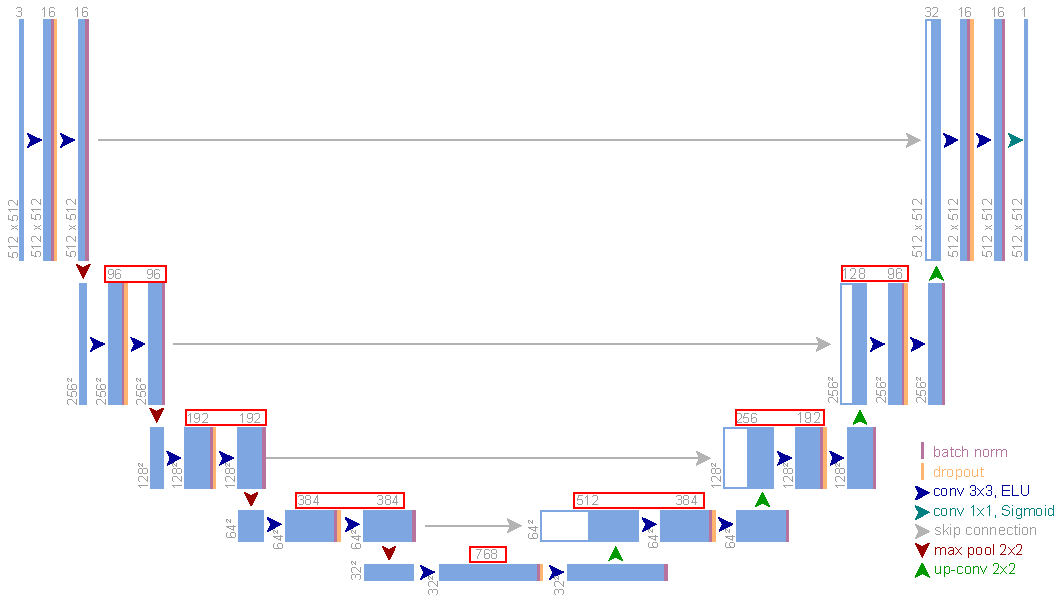
\includegraphics[width=1.\textwidth]{Bilder/own-unet-15mil-marked.pdf} 
	\caption{Bike-U-Net-15 mit 15,165 Mio. Parametern. Die geänderten Convolution-Filteranzahlen sind mit roten Kasten markiert.}
	\label{fig:bike-unet-15}
\end{figure} 

\begin{itemize}
	\item Zunächst werden Input-Bilder der Größe $width \times height \times 3$ verwendet. 
	Wobei $width$ und $height$ variabel in der Architektur sind, mit der Einschränkung, 
	dass diese Vielfache von 32 sein sollen, damit die mittlere Schicht nicht zu klein wird. 
	In jedem Fall wird ein Bild mit drei Kanälen (RGB) verwendet. 
	In der Abbildung ist exemplarisch $512 \times 512 \times 3$ gewählt. \\
	Der Output verwendet lediglich ein Output-Neuron pro Input-Pixel, wobei keine Aktivierung einen Hintergrundpixel 
	und eine Aktivieriung einen Radweg-Pixel impliziert, wie in \autoref{sec:state-of-the-art-roads} beschrieben. 
	\item Bei den Convolutional-Layern wird Padding eingesetzt,
	um die Dimensionen der Feature-Maps nicht nach und nach zu verkleinern und so einen exakt symmetrischen Aufbau zu gewährleisten.
	Ebenso wurde bei den Up-Convolutions Padding eingefügt, um auch hier eine Verkleinerung der Feature-Maps zu verhindern.
	Diese Anpassung wurde eingesetzt, um kein Zuschneiden bei den Skip-Connections zu benötigen, was die Lokalisierung verbessern soll,
	und so bei den in \autoref{sec:state-of-the-art-roads} beschriebenen Netzen gewöhnlich ist.
	\item 
	Im Bike-U-Net-2 beginnen die Filter bei 16 und verdoppeln sich bis 256, was zu ungefähr 2 Mio. 
	trainierbaren Parametern führt. Die Zahl an Parametern ist somit weitaus geringer als im 
	Original-U-Net (vgl. \autoref{sec:architekturkomponenten:unet}). \\
    Das \textit{\acf{BUNet15}} hat 15 Mio. Parameter (\autoref{fig:bike-unet-15} zeigt \ac{BUNet15}). Dies wird erzielt, 
	indem die Filteranzahl ab dem zweiten Block dreimal höher ist als in \ac{BUNet2}. So sind hier 16 Filter in Block eins, 
	dann 96 Filter in Block zwei, die sich verdoppeln bis hin zu 768 Filtern im mittleren Block und danach wieder halbieren bis zum vorletzten Block. 
	Dabei hat der letzte Block wieder 16 Filter. 
	Der erste und letzte Block haben jeweils 16 Filter, da damit der Rechen- und Speicheraufwand erheblich reduziert werden kann.
	Bis auf die Filteranzahl und die daraus resultierende Tiefe der Feature-Maps, sind \ac{BUNet2} und Bike-U-Net-15 identisch.
	\item Auf jede Convolution-Schicht folgt eine Batch-Normalization-Schicht. 
	\item Zusätzlich zu den Batch-Normalization-Schichten werden pro Block eine Dropout-Schicht 
	nach der jeweils ersten Convolution-Schicht eingezogen. Diese eröffnen den in \autoref{sec:hyperparameter:dropout} 
    beschriebenen Hyperparameter \textit{Dropout-Rate}.
	\item Die Convolution-Schichten werden durch \ac{ELU} (s. \autoref{sec:activation:elu}) aktiviert, 
	anstatt durch \ac{ReLU}, wie im Original-U-Net. 
	Hierdurch können die meisten der in \autoref{sec:activation} herausgearbeiteten Vorteile von \ac{ReLU},
	wie Robustheit gegen das Vanishing-Gradient-Problem, genutzt werden.  
	Um das Dying-Neuron-Problem zu adressieren, welches zu den in \autoref{sec:architekturkomponenten:unet} genannten Problemen führt, 
	wird auf \ac{ELU} (s. \autoref{sec:activation:elu}) zurückgegriffen, da damit alle Netzteile aktiv bleiben sollen. 
	Nachteil ist hierbei, dass die Berechnung von \ac{ELU} etwas aufwendiger ist. 
	Das Problem von unbeschränkt großen positiven Aktivierungen unter denen sowohl \ac{ELU} als auch \ac{ReLU} leiden,
	wird in diesem Netz durch die wiederholte automatische Standardisierung und Normalisierung durch die Batch-Norm-Schichten abgefedert.
	\item Für das Ouptut-Layer, nach der $1\times 1$-Convolution, wird die Sigmoid-Funktion verwendet. 
\end{itemize}

\subsection{VGG16-Bike-U-Net}

\textit{\ac{VBUNet}} nutzt das in \autoref{sec:pretrained-backbones:vgg16} beschriebene Netz VGG16 
mit auf ImageNet vortrainierten Gewichten als Backbone. \\
Hierzu werden die drei Fully-Connected-Layer 
(und Soft-Max-Aktivierung) am Ende entfernt und mit drei neuen \textit{conv3-512}-Schichten ersetzt. 
Diese bilden den mittleren (\enquote{untersten}) Block im U-Net. Darauf folgt eine direkte Spiegelung 
von VGG16 als Decoder mit abschließender $1\times 1$-Convolution. Im Gegensatz zum Bike-U-Net (s. \autoref{sec:architecture:bike-u-net}) 
und ursprünglichen U-Net (s. \autoref{sec:architekturkomponenten:unet}) werden allerdings keine 
\textit{Up-Conv3}-Layer mit trainierbaren Gewichten zum Upsampling genutzt, sondern 2D-Upsampling-Layer, 
ohne trainierbare Parameter. Diese Entscheidung wird getroffen, um VGG16 besser nachzuempfinden, 
da hier Maxpool-Schichten zum Downsampling verwendet werden, die ebenfalls keine trainierbaren Parameter enthalten.
Weiterhin sind nach jeder nicht-vortrainierten Convolution-Schicht, also nach jeder, die nicht zu VGG16 gehören, 
Batch-Normalization-Layer eingezogen, aus den in \autoref{sec:architecture:bike-u-net} und \autoref{sec:architekturkomponenten:batchnorm}
genannten Gründen wie schnellerem Training, leichter Glättung und fehlender sonstiger Standardisierung und Normalisierung.
Die für U-Net charakteristischen Skip-Connections werden vor jeder Maxpool-Schicht außer der ersten eingesetzt 
und mit dem korrespondierenden Decoder-Block verbunden. Dies resultiert in genau vier Skip-Connections, 
wie im Bike-U-Net und originellen U-Net. Abgeschlossen wird durch eine Sigmoid-Aktivierung, so wie im Bike-U-Net. \\
VGG16-Bike-U-Net enthält 23,7 Mio. Parameter. Grob die Hälfte davon (14,7 Mio.) sind von VGG16. 

\subsection{ResNet34-Bike-U-Net}

\textit{\ac{RBUNet}} nutzt das in \autoref{sec:pretrained-backbones:resnet} beschriebene Netz ResNet34 
mit auf ImageNet vortrainierten Gewichten als Backbone. 
Hierzu wird die eine Fully-Connected-Layer am Schluss des Netzes entfernt und mit einem Decoder ersetzt. 
Anders als bei \ac{VBUNet} ist der mittlere Block der U-Net-Struktur von ResNet34 
und nicht zusätzlich neu ergänzt. Grund dafür ist die höhere Anzahl an Parametern 
von ResNet34, welche ohne die Fully-Connected-Schicht bereits bei 24,4 Mio. liegt, im Gegensatz zu VGG16. 
Da der mittlere Block die meisten Parameter beinhaltet, wird keine weitere Vertiefung des Netzes vorgenommen,
um die Anzahl der Parameter nicht drastisch zu erhöhen. Anstelle dessen wird nach Ende der Convolution-Schichten von 
ResNet34 direkt mit dem Upsampling begonnen, welches wie bei \ac{VBUNet} mit Upsampling-Schichten 
bewerkstelligt wird. Auch wird im Widerspruch zu \ac{VBUNet} der Encoder - also ResNet34 - nicht gespiegelt, 
um eine Verdoppelung der Parameteranzahl zu vermeiden. Stattdessen wird ein einfacher, U-Net-ähnlicher Decoder
aus fünf Blöcken á Upsampling-Schicht und zwei Convolution-Schichten verwendet, wobei in jedem Block 
die Filter-Anzahl von 512 an bis schließlich 16 halbiert wird. Abgeschlossen wird wie bei \ac{VBUNet} und
\ac{BUNet} mit $1\times 1$-Convolution und Sigmoid-Aktivierung. Aus den gleichen Gründen wie bei \ac{VBUNet}
sind nach jeder Convolution-Schicht Batch-Normalization-Schichten eingezogen. 
Es erfolgt wiederum das Einsetzen von vier Skip-Connection nach U-Net-Vorbild ergänzend zu den 
Skip-Connections der Residuen-Blöcke an folgenden Stellen: 
nach der $7\times 7$-Convolution zu Beginn von ResNet34, 
am Ende der Blöcke mit 64 Filter, am Ende der Blöcke mit 128 Filtern 
und am Ende der Blöcke mit 256 Filtern. Im Decoder werden diese jeweils 
zu Beginn der ersten vier Decoder-Blöcke konkateniert. \\ 
ResNet34-Bike-U-Net enthält 24,4 Mio. Parameter. Davon sind 21,2 Mio. von ResNet34 und lediglich 3,2 Mio. 
vom Decoder, welcher somit eher unterrepräsentiert ist im Netz.  

\subsection{DenseNet121-Bike-U-Net}

\textit{\ac{DBUNet}} nutzt das in \autoref{sec:pretrained-backbones:densenet121} beschriebene Netz DenseNet121 
mit auf ImageNet vortrainierten Gewichten als Backbone.
Hierzu wird der Classification-Layer bestehend aus einer $7\times 7$-Average-Pool-Schicht 
und einer Fully-Connected-Layer entfernt und durch einen Decoder ersetzt. 
Wie schon bei \ac{RBUNet} erstreckt sich das DenseNet bis in den mittleren U-Net-Block. Beim \ac{DBUNet} 
liegt der Grund dafür allerdings nicht in der hohen Parameterzahl, sondern in der hohen sonstigen Komplexität 
des Netzes. So benötigt DenseNet121 trotz deutlich geringerer Parameterzahl für die Inferenz und das Training länger 
als sowohl \ac{RBUNet}, als auch \ac{VBUNet}. Vermutlich ist hierfür die große Tiefe von 64 Schichten, wovon 
60 Convolution-Schichten sind, verantwortlich. Um die Inferenz- und Trainingszeit nicht weiter zu belasten, 
ist der Decoder eher simpel gehalten, enthält also wenig Parameter. Für den Decoder wird die gleiche Architektur wie im \ac{RBUNet} verwendet.
Auch hier sind die Batch-Normalization-Schichten eingezogen. Der Unterschied besteht darin, 
dass die erste Convolution-Schicht anders als bei \ac{RBUNet} nicht von 512 Kanälen auf 256 abbildet, 
sondern von 1536 auf 256. Dies liegt an der Konkatenierung der DenseNet-Architektur. Wieder wird das 
Netz abgeschlossen durch eine $1\times 1$-Convolution gefolgt von einer Sigmoid-Aktivierung. 
Auch hier werden wieder vier Skip-Connections eingebaut, um die U-Net-Architektur nachzuahmen. 
Diese Skip-Connections sind im Falle von \ac{DBUNet} im Encoderteil nach der ersten $7 \times 7$-Convolution 
und dann jeweils nach jeder weiteren $1\times 1$-Convolution der DenseNet-Transition-Zonen eingesetzt. 
Im Decoder-Teil sind diese wie bei \ac{RBUNet} zu Beginn jedes Decoder-Blocks bis auf den letzten eingebaut. \\
DenseNet121-Bike-U-Net enthält 12,1 Mio. Parameter, wovon 6,9 Mio. zum DenseNet121 und 5,1 Mio. neu hinzugefügt 
wurden. Trotz doppelter bzw. sogar vierfacher Tiefe besteht \ac{DBUNet} nur aus ungefähr halb so vielen 
Parametern wie \ac{RBUNet} und \ac{VBUNet}. 


% Zunächst wird eine Basisimplementation gegeben, die den Algorithmus zur Subproblemerzeugung und Similarity-Berechnung aus \autoref{sec:alg_comp} umsetzt und diesen dann auf Geschwindigkeit optimiert.

% \section{Basisimplementation}

% \begin{algorithm}
% 	\caption{Vereinfachter Algorithmus zum Erstellen der Subprobleme aus den Submodellen}\label{lst:create_sub}
% 	\begin{algorithmic}[1]
% 		\Procedure{Create Subproblems}{$F$} 
% 			\For{$S \in atomicSubmodels$}
% 				\State $S.graph \gets calculateGraph(S)$
% 				\State $S.graph \gets reduceGraph(S.graph, F)$
% 			\EndFor \Comment{$n := |atomicSubmodels|$}
% 			\While{$|atomicSubmodels| \neq 0$} \Comment{$O(\frac{n(n+1)}{2}) \cdot O(t_{sim}) = O(n^2 \cdot t_{sim})$}
% 				\State $M \gets selectOne(atomicSubmodels)$
% 				\State $M.set \gets \emptyset$
% 				\While{$complexity(M) < minSubproblemComplexity$}
% 					\State $highestSim \gets -1$					
% 					\For{$S \in atomicSubmodels$}
% 						\State $sim \gets computeSim(M, S)$
% 						\If{$sim > highestSim$}
% 							\State $mostSimilar \gets S$
% 							\State $highestSim \gets sim$
% 						\EndIf
% 					\EndFor
% 					\State $M \gets M \cup mostSimilar$
% 					\State $M.set \gets M.set \cup mostSimilar.set$
% 					\State $atomicSubmodels \gets atomicSubmodels \setminus mostSimilar$
% 				\EndWhile
% 				\State $subproblems \gets subproblems \cup \{M\}$
% 			\EndWhile		
% 		\EndProcedure
% 	\end{algorithmic}
% \end{algorithm}

